\documentclass{sig-alternate}
\usepackage{graphicx}
\usepackage{url}

\begin{document}

\title{NetFl.ux: Visualizing Netflow Data Using Modern Web Technologies}
\subtitle{Dept. of CIS - Senior Design 2013-2014
    \thanks{Advisor: Boon Thau Loo (boonloo@cis.upenn.edu)}}
\author{Patrick Wingo\\ \email{pbwingo@gmail.com}\\ Univ. of Pennsylvania
    \and Aubrey Chase\\ aubchase@seas.upenn.edu\\ Univ. of Pennsylvania
    \and Bill He\\ billshihe@gmail.com\\ Univ. of Pennsylvania
    \and Daniel Ge\\ dange@seas.upenn.edu\\ Univ. of Pennsylvania
    \and Ryan Sasson\\ rsasson@seas.upenn.edu\\ Univ. of Pennsylvania}

\maketitle

\section*{Abstract}

We propose to create a tool to help Penn system administrators better understand
the health and security of their network.  Current networking protocols and
tools present data in a way that is too disaggregated and computer-driven to
understand. We plan to leverage LLDP (Link-Layer Discovery Protocol), SNMP
(Simple Network Management Protocol), as well as NetFlow (packet metadata
inspection) as data sources. In order to more effectively visualize and analyze
the data, we plan to use modern web technologies such as MapReduce for
real-time, large-scale computation, as well as node.js in order to
asynchronously update data between the server processing network data and the
client displaying it.

Our product will differentiate itself on three primary attributes: real-time
analytics enabled through distributed computation, cross-platform compatibility
because of our display through traditional web browsers, as well as focus on
user experience to enhance the analytical abilities of the user. We aim to
create a tool to allow administrators to quickly understand problems at a macro
level, then to easily drill down and display potential problems at the component
level to speed the manual network diagnostics process.

\section*{Glossary}

\textbf{Link Layer Discovery Protocol (LLDP)} is a protocol used to discover the
topology of a network. This protocol allows Ethernet devices such as routers and
bridges to broadcast information about themselves such as capabilities and
neighbors, as well as receive this information from other devices.  Ethernet
devices broadcast information about themselves, store information they learn
about each other in local databases, and a network management system accesses
this data to build a map of the network topology. The basic unit of data
transmitted by this protocol is a LLDP Protocol Data Unit (PDU). A LLDP PDU
consists of a header followed by elements known as TLVs (Type, Length, Value).

\textbf{NetFlow} is a protocol used for collecting and analyzing network
traffic. On a high level, a flow is a series of packets that are similar to each
other. More specifically, we will be working with Cisco's Version 5 and Version
9 flow records where a flow is defined by source IP address, destination IP
address, source port number, destination port number, layer 3 protocol type, ToS
byte, and input logical interface. Each flow consists of a flow header, which
contains information such as Netflow version and number of records, and flow
records, which contains information such as source and destination IP, bytes,
and IP protocol. Netflow is sent from routers and switches to a collector
machine where it can be stored, exported, and/or used for analysis.

\section{Introduction}

Many IT professionals are required to perform analysis of a computer network to
discover information such as percentage of traffic used by certain applications,
which users use the network the most, how usage patterns have changed over time,
and the geographic patterns of network connections. LLDP, SNMP, and Netflow data
have emerged as a protocols to perform this analysis and tools such as NFSen
have enabled visualization capabilities by enabling users to look at the data in
a variety of forms such as logs, charts, and graphs.

We believe that existing tools can be improved upon. Log files give extremely
granular detail that provides rich information, but can be overwhelming for a
user. Charts give a high level picture of network statistics, but sacrifice
detail to achieve that simplicity. Existing graph solutions offer a logical and
intuitive way of viewing a network, but fail to incorporate both high level
visualization and low level detail elegantly into one workspace. Furthermore,
existing tools mainly focus on network forensics, but offer little in the way of
incident detection.

We hope to create a network visualization tool that addresses these problems.
Our tool will combine log, chart, and graph visualization methods to
simultaneously offer users a high-level picture of the network and node-level
detail in one workspace. To further enhance the analysis capabilities of users,
we will also incorporate event detection to detect events such as traffic spikes
and security threats to make our system proactive. These capabilities will be
enhanced by performing the analysis in real-time and making our system web-based
and multi-platform.

\section{Related work}

Much software has been written to improve the utilization of NetFlow for network
analysis and visualization, and there are a variety of open- and closed-source
tools available. The same applies for SNMP and LLDP tools. In fact, LLDP is
specifically designed in order to provide information on the topology of a
network, the very thing that we want to first build out, but we find that the
tools are widely disaggregated, and often unintuitive to use. For example, LLDP
is a command line based tool, so that the results output is completely
text-based, and even after reading manuals, it was difficult to understand the
output.

One of the best software packages we found was solarwinds, which is a very
expensive NetFlow analysis package, which breaks down network nodes in tree
form, on a map, by CPU usage, node health, and other metrics. We found that it
was a great way to diagnose potential problems with the network, but based on
our test of the free trial, were unable to find out the exact problem. The user
interface was also somewhat confusing: the relationship between different
metrics and graphs was not highlighted. In addition, it appears that LLDP and
SNMP were not incorporated into the solarwinds software; we believe that by
integrating multiple data sets, we can provide a more holistic picture of
network health.

Another tool we looked into was nfsen, an open-source web-based NetFlow
aggregator and analyzer. It took raw NetFlow data from another open-source tool,
nfdump, and visualized it onto a web interface. It solved the problem of
cross-platform visualization, but the graphs are too high-level to be useful for
anything other than knowing there was a problem. We spoke with the Penn system
administrators, and they found nfsen to be useful only in detecting potential
anomalies. From there, they used command tools and sometimes a multitude of
other software platforms in order to understand the problem in detail.

Work by Minarik and Dymacek\cite{Minarik08} demonstrated a clear understanding
of the need for system administrators to be able to intuitively understand a
problem using a graph-based, high-level examination, then to drill down on those
nodes and understand statistics for those nodes in order to further
investigate.They even included programmatic DNS, port, and WHOIS lookups in
order to reduce the mechanical work of an analyst, but we found that they didn’t
use LDDP or SNMP in order to create and understand topology, and their user
interface looked like it could use some improvement as the usage case was not
entirely intuitive.

In terms of work to understand campus wireless networks, we found that Kotz et
al.\cite{Kotz05} used SNMP in order to understand macro-scale campus networks
as wireless was emerging in 2005. Although the research primarily investigated
roaming across the network, which is not entirely relevant to our proposed work,
their method of breaking down traffic across the network using SNMP is relevant.
The researchers polled their access points every 5 minutes using the SNMP
software installed across the network, and got inbound/outbound byte counts as
well as recent MAC addresses. From there, they were able to graph out traffic
over the course of an average day as well as traffic patterns over a long period
of time.

Yin et al.\cite{Yin04} developed a tool called VisFlowConnect which is a
visualization tool that uses a parallel axes representation of Netflow to help
users visualize network traffic. The development of VisFlowConnect was motivated
by the insufficiency of traditional tools to present hostile attack patterns in
an intuitive way for the human mind.  VisFlowConnect has various features that
have served as inspiration for our project, including interface views of
different granularity (e.g. global, intra-network) and filtering of data on
various parameters (e.g. protocol, packet-size). However, a shortcoming of
VisFlowConnect is the inability to drill down on the flow data and not only
filter on, but observe information such as protocol and transfer rate. In
addition, we feel that a parallel axes representation of the network can be
somewhat overwhelming and unintuitive and that a graph representation would be
better.

Ball et al.\cite{Ball04} developed a tool called Visual Information Security
Utility for Administration Live (VISUAL) which allows users to see communication
patterns between internal networks and external hosts in a graphical
representation.  After surveying IT professionals, Ball, Fink, and North found
that users found it difficult to quickly assess the security state of networks
with text-based tools. They found that with VISUAL, users could develop insights
from the traffic data without any training, demonstrating the power of
visualization tools. VISUAL's main features include markers for external and
internal hosts, color-coded links between external and internal hosts,
interactive filtering, and time lines. Shortcomings of VISUAL that we hope to
address include more proactive displays (e.g. having an internal host flash red
when there's a traffic spike) and processing network data in closer to
real-time.

\section{Proposed work}

The architecture of the application can be broken down into 3 main components: a
module that collects netflow data from the network, network data processing and
storage within the cloud (most likely AWS), and a web front end to all of the
processed data.

The first challenge we anticipate is simply the sheer volume of the LLDP data
(and eventually Netflow if time is permitting) the collector will need to
collect and transfer over to the data processor in the cloud. This volume could
easily reach the scale of terabytes if collected for long enough. We will devise
a way to take this volume of data and stream it to the processing cluster in the
cloud. Transferring this high volume of data to a cloud service could be
potentially costly so we will need to consider ways to keep this cost low and
transfer the data efficiently. If we reach the point where we work with Netflow
data we must address security and privacy concerns with this collection. Most
likely we will need to anonymize the network data before we send it over to the
data processor.

\begin{figure}[htb!]
    \centering
    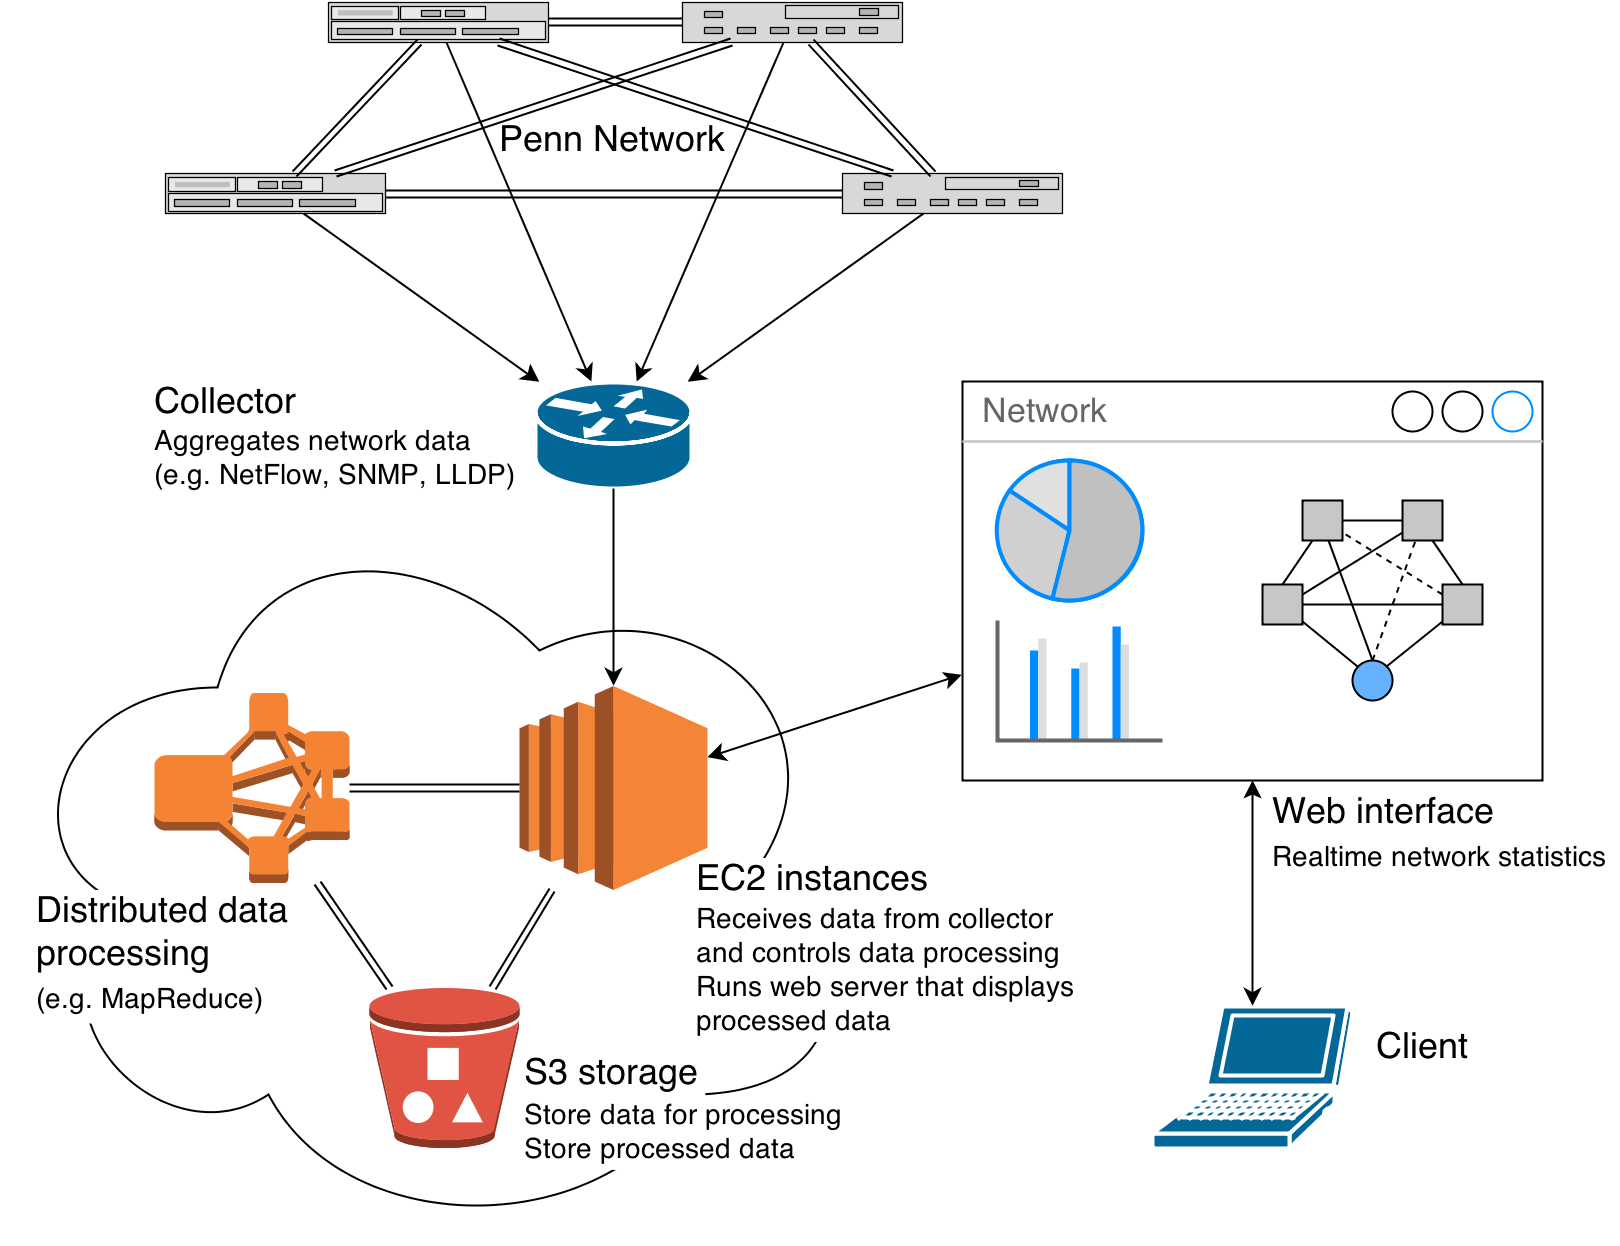
\includegraphics[width=\linewidth]{mockup}
    \caption{Proposed architecture of the project}
    \label{fig:mockup}
\end{figure}

Within the cloud we will host the data processing module (likely using Hadoop or
another horizontally scalable data processing framework). Within this module
there are 3 main components (data processor, index to stored data, and server
for web application). The data processor will apply the necessary aggregations
to make the data set manageable for later indexing (We are looking to apply more
sophisticated analysis on the data if time permits). All this data will be
stored in an easily accessible and queryable database (likely some form of a SQL
database or a distributed SQL database if the data set is large) so the web
frontend server can query it when rendering HTML pages. The web server will
serve the frontend application to the requesting user.

For the web front end we will provide the user a clear and insightful view into
the network data. We will use modern web UI frameworks that leverage HTML, CSS,
and JS so that this application will look consistent among multiple platforms.

\section{Timetable}

Milestones

\bibliographystyle{plain}
\bibliography{sources}

\nocite{*}

\end{document}
